\section{Exercise 3: Signal Generator Circuit Analysis}

\subsection{Objective}
The purpose of this exercise is to learn how to use signal generator and ossiloscope. 

\subsection{Equipment}
\begin{itemize}
    \item Signal Generator (w/ equipments)
    \item Oscilloscope (w/ equipments)
    \item Breadboard
    \item Wires (Jumper Cables \& Crocodile Clips)
    \item Resistors ($1k\Omega$, $4.3k\Omega$)
\end{itemize}

\subsection{Procedure}
\begin{enumerate}
    \item We have made the circuit analysis using LTspice and these are the results:  
    \begin{figure}[h]
        \centering
        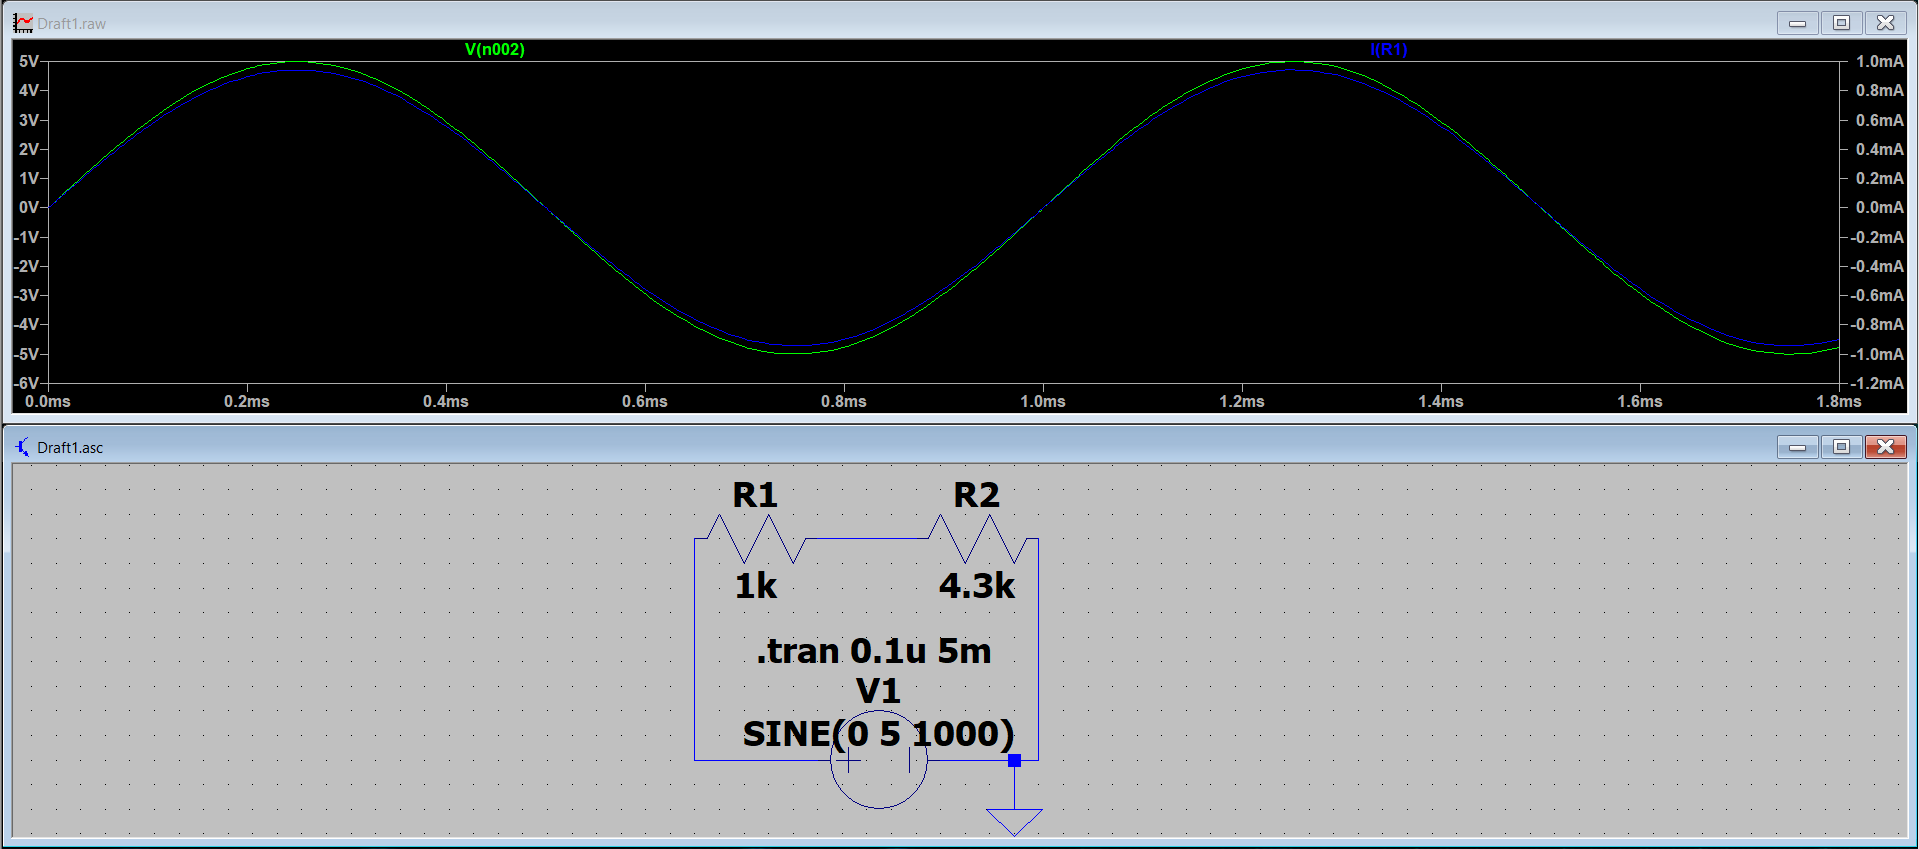
\includegraphics[width=1\textwidth]{assets/taks_3.png}
        \caption{Circuit Diagram \& Calculations}
    \end{figure}

    \newpage
    \thispagestyle{plain}

    \item We have connected the resistors in series on the breadboard as shown in the figure below:
    \begin{figure}[h]
        \centering
        \begin{circuitikz} \draw
            (0, 7) to[sinusoidal voltage source, l=5V~1kHz] (0, 0)
            (0, 7) to[R, l=$1k\Omega$] (7, 7)
            (7, 7) to[R, l=$4.3k\Omega$] (7, 0)
            -- (0, 0);
        \end{circuitikz}
        \caption{Series Circuit with Two Resistors}
    \end{figure}

    \newpage
    \thispagestyle{plain}

    \item We have connected the signal generator to the circuit and measured the voltage using the oscilloscope. These are the results:
    \begin{figure}[h]
        \centering
        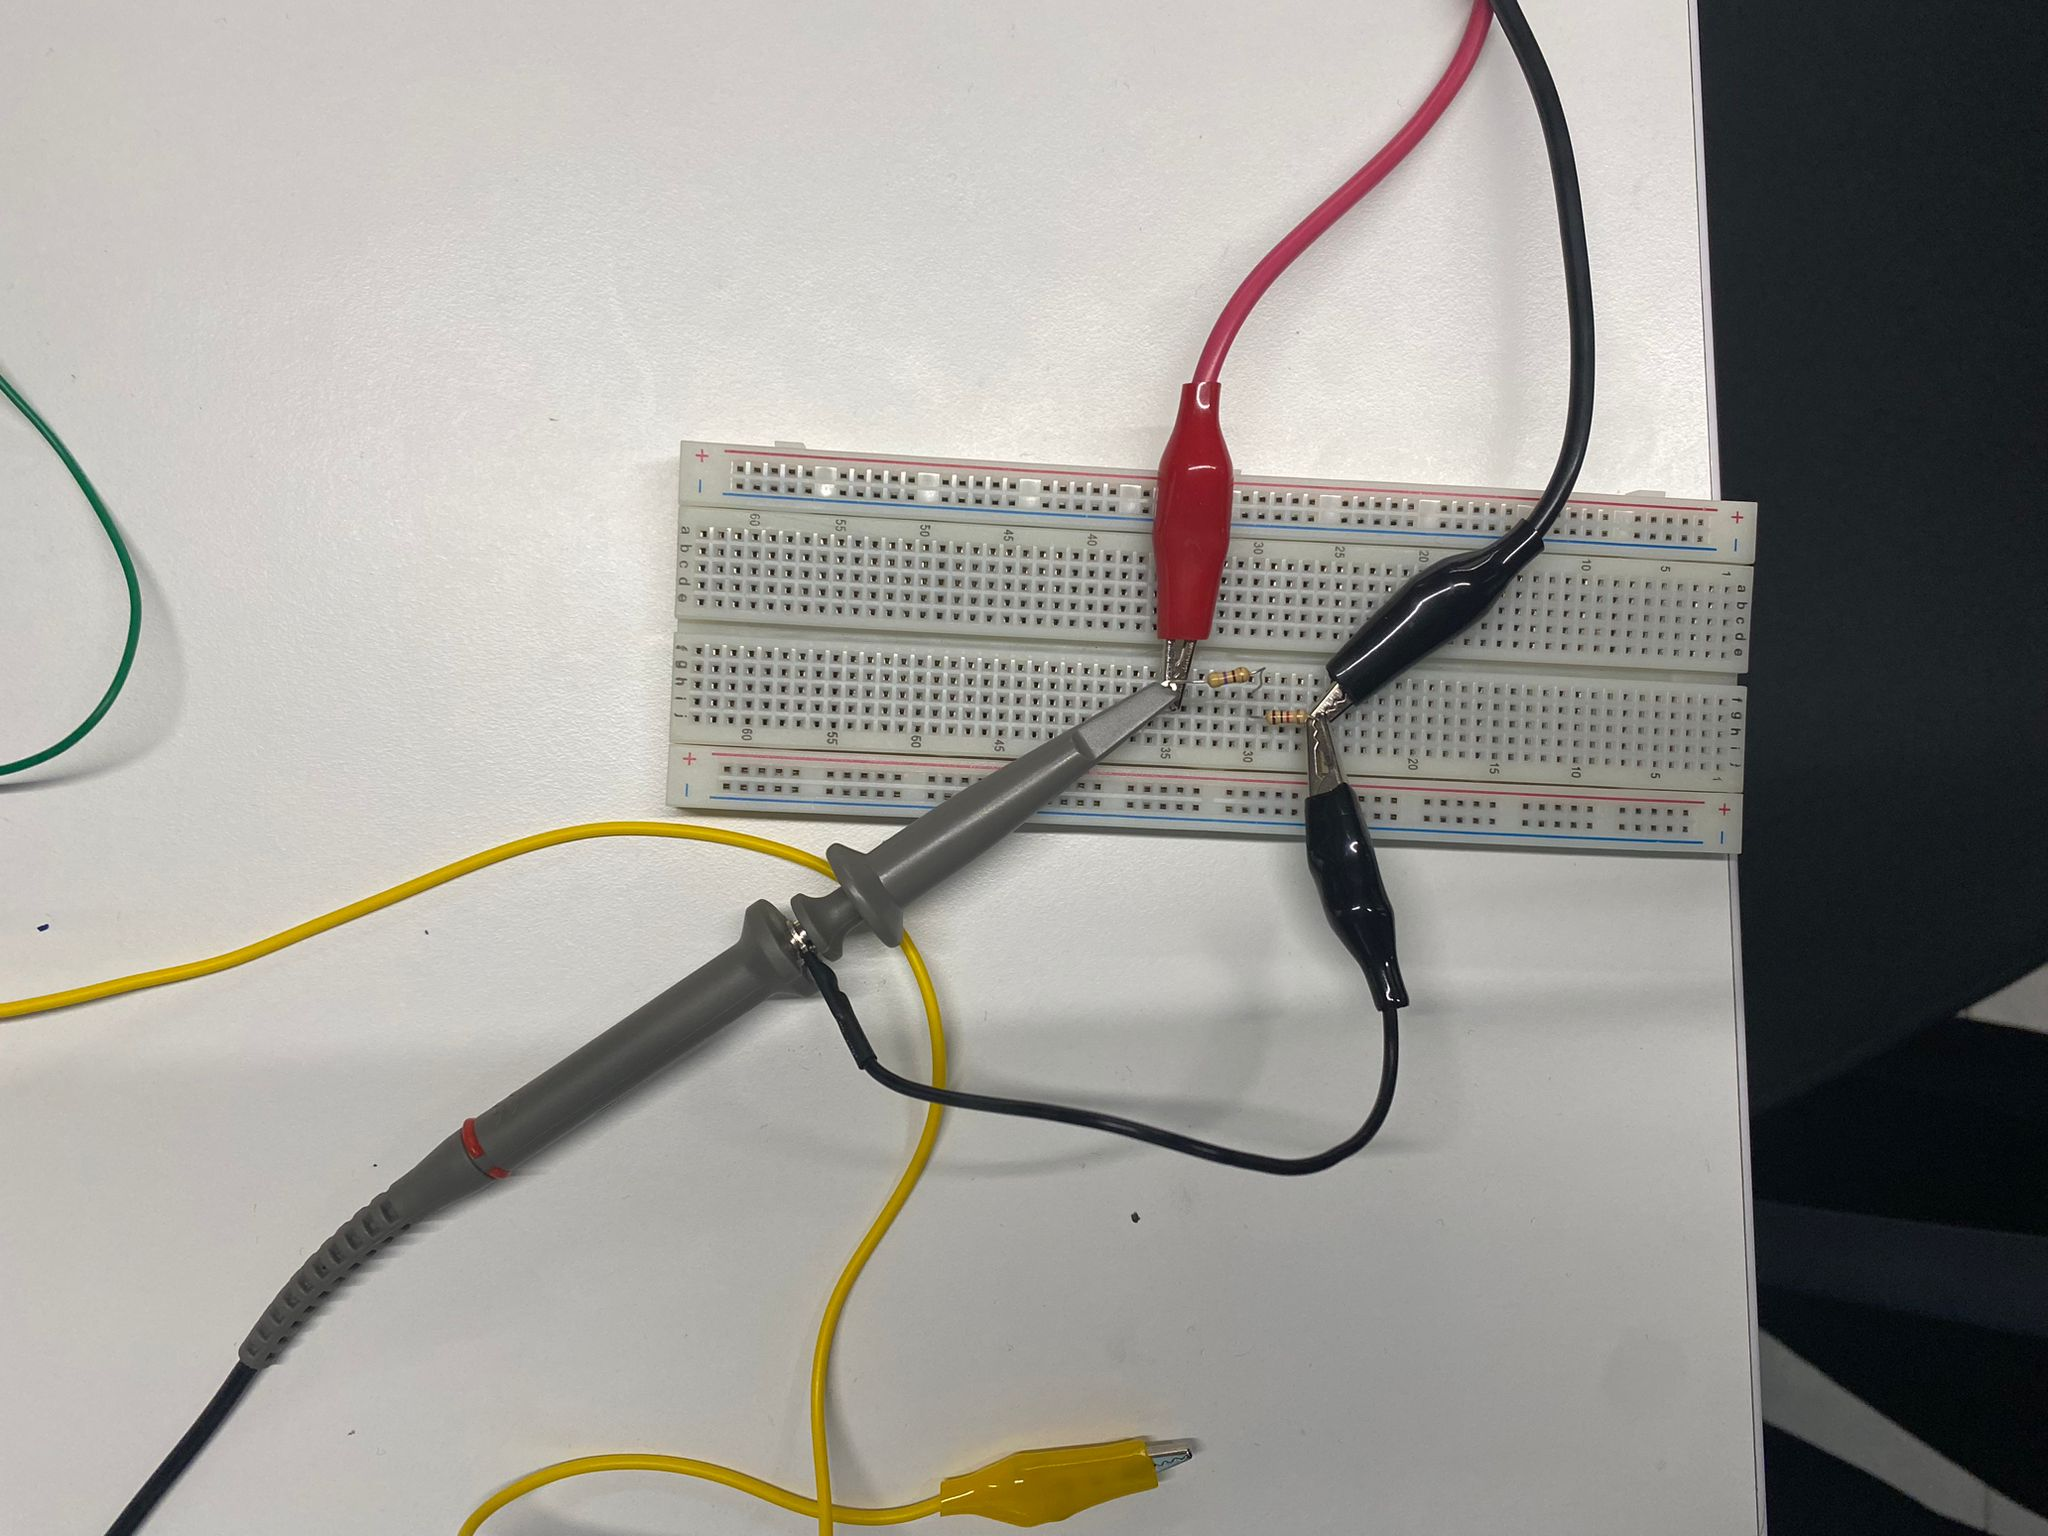
\includegraphics[width=.75\textwidth]{assets/IMG-20240307-WA0018.jpg}
        \caption{Oscilloscope Probe Connection}
    \end{figure}
    
    \begin{figure}[h]
        \centering
        \begin{minipage}{.5\textwidth}
            \centering
            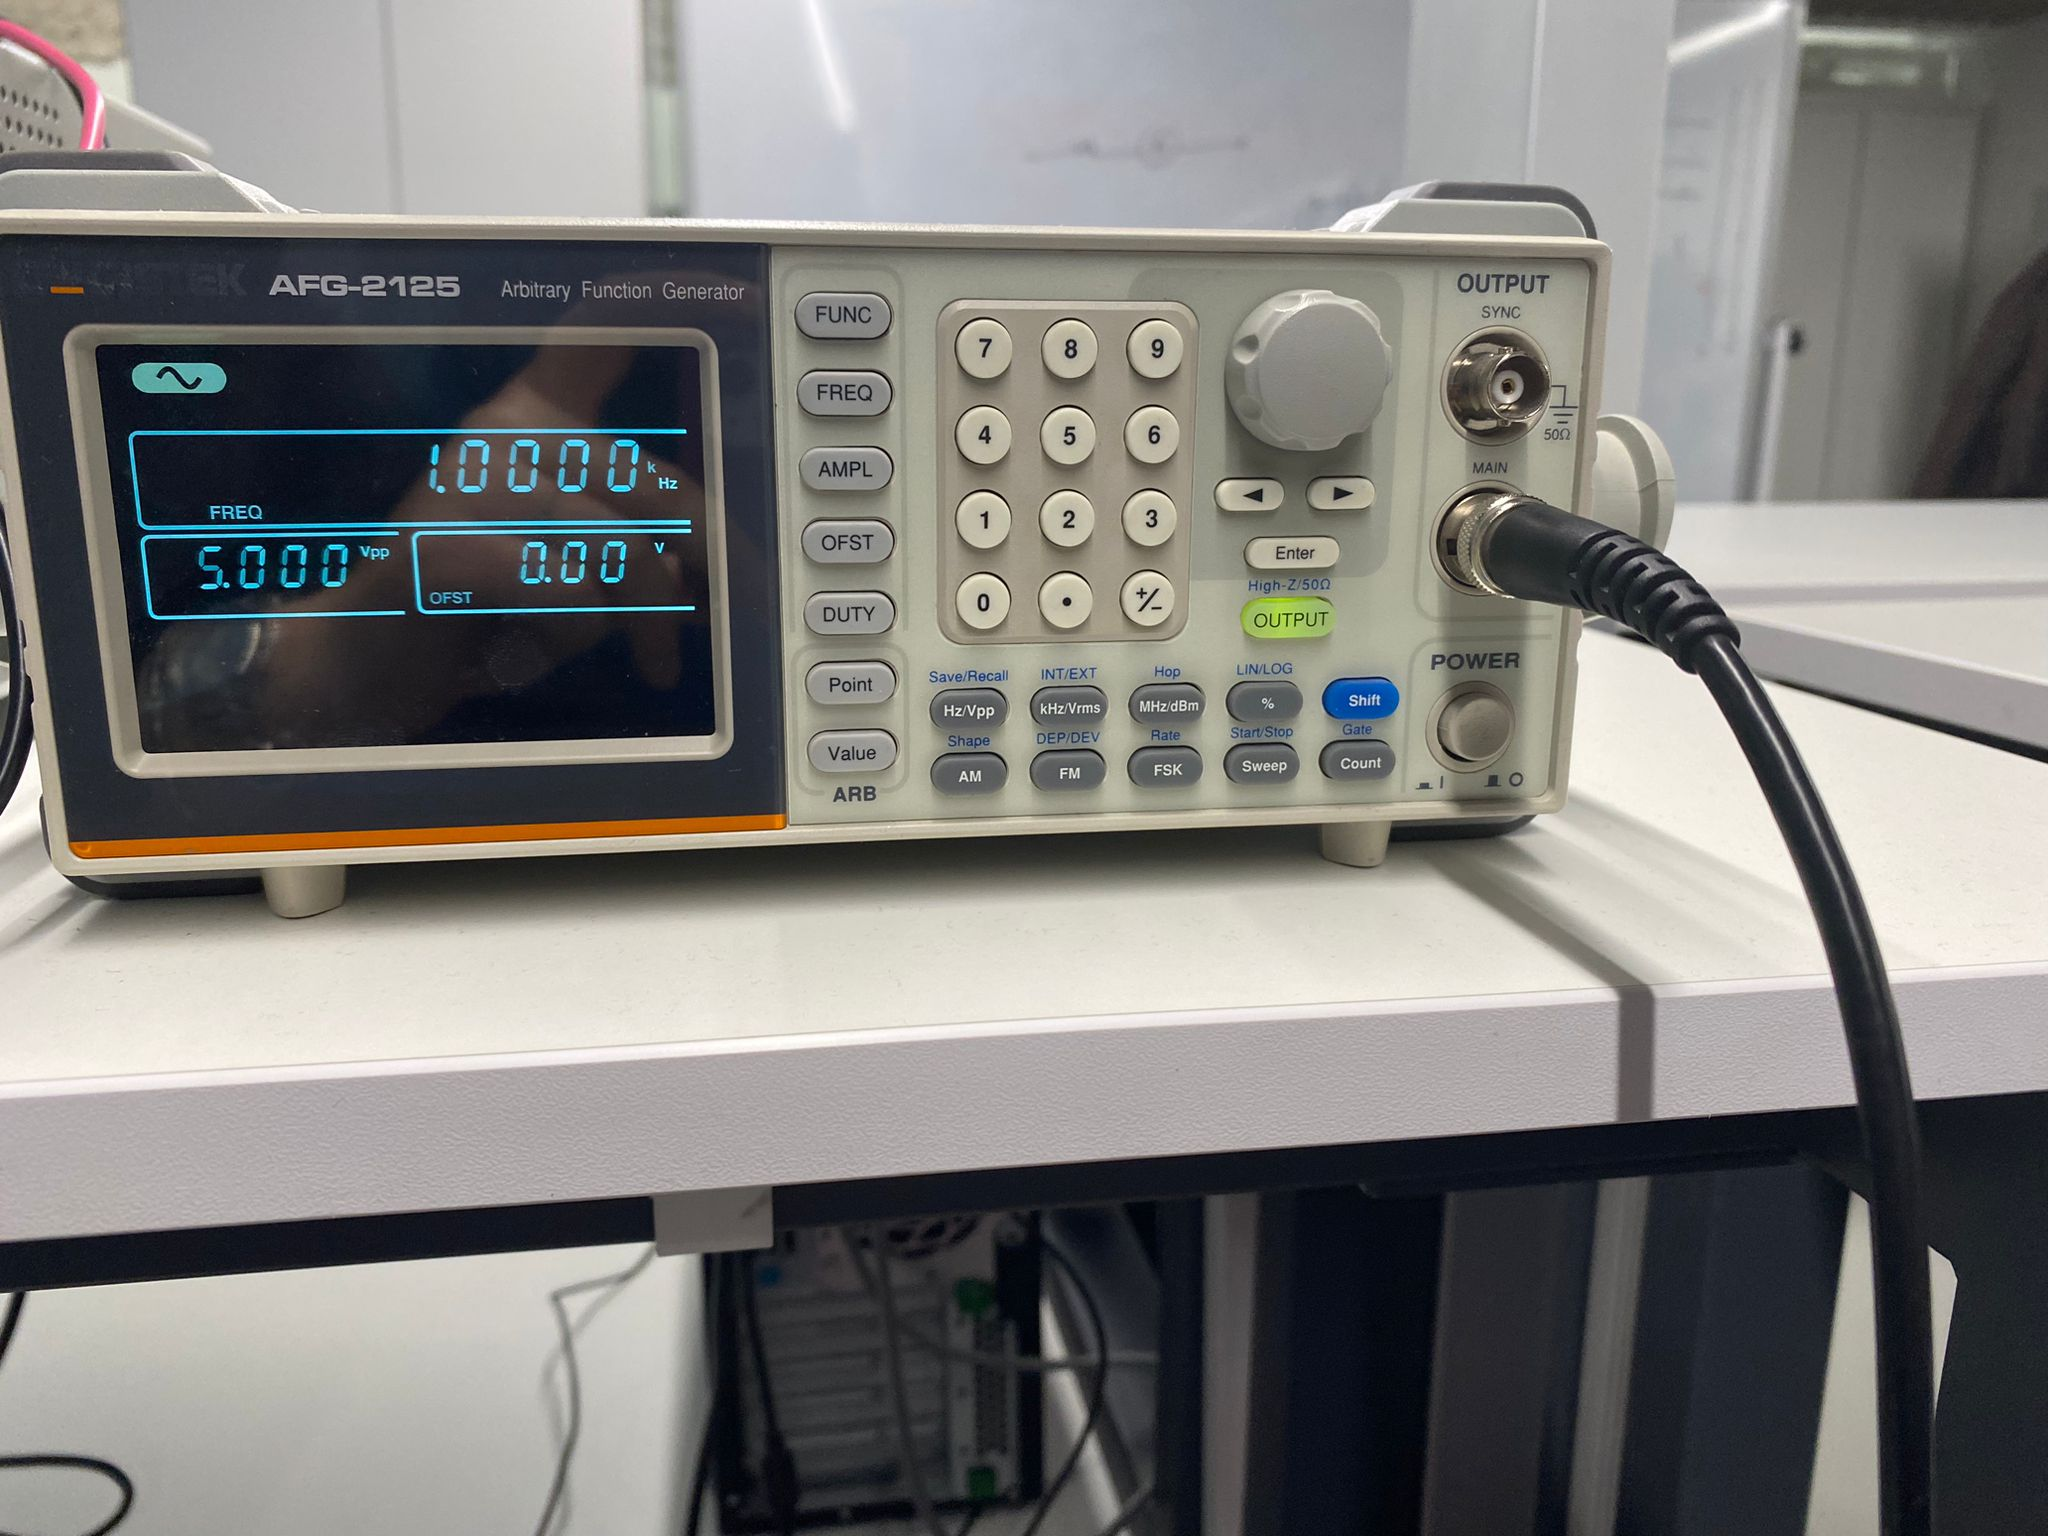
\includegraphics[width=.9\linewidth]{assets/IMG-20240307-WA0010.jpg}
            \captionof{figure}{Signal Generator Set To Sinusodial@5V~1kHz}
        \end{minipage}%
        \begin{minipage}{.5\textwidth}
            \centering
            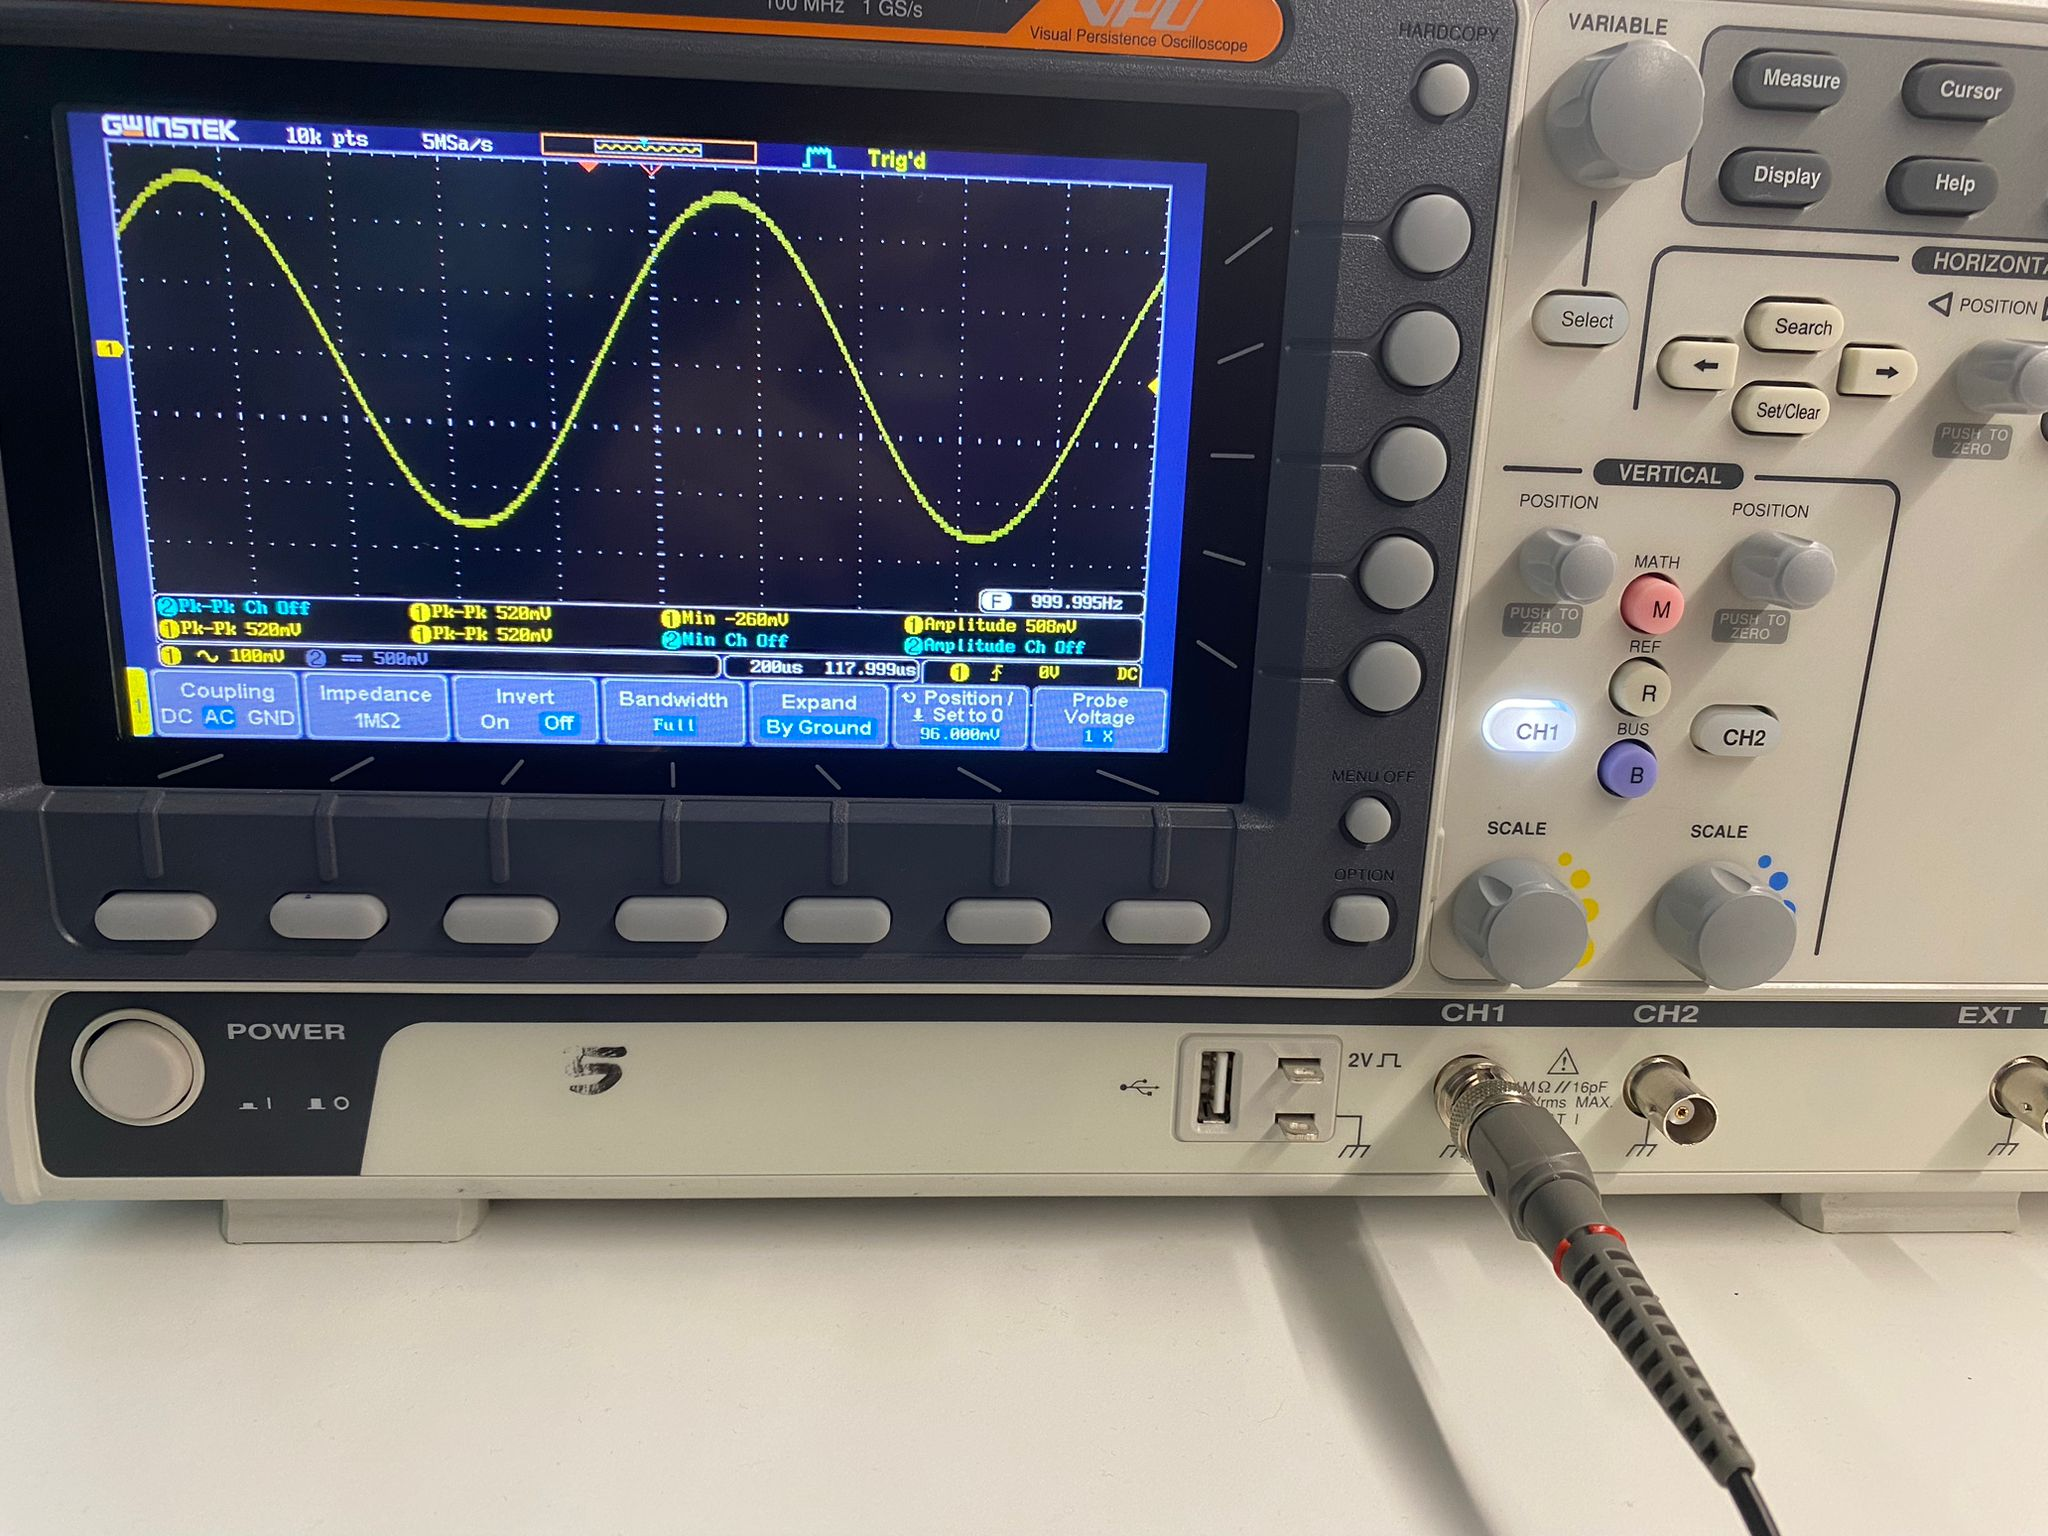
\includegraphics[width=.9\linewidth]{assets/IMG-20240307-WA0017.jpg}
            \captionof{figure}{Oscilloscope Measurement Results} 
        \end{minipage}
    \end{figure}
\end{enumerate}

\subsection{Results}
We have successfully measured the voltage of the circuit using the oscilloscope. The measured voltage is close to the expected value. The differences between the expected and measured values are due to the tolerance of the resistors and the measurement errors.

\newpage
\thispagestyle{plain}
